\documentclass[a4paper,12pt]{article}
\usepackage[utf8]{inputenc}
\usepackage[MeX]{polski}
\usepackage{fixltx2e}
\usepackage[table,xcdraw]{xcolor}
\usepackage[utf8]{inputenc}
\usepackage[T1]{fontenc}
\usepackage{graphicx}
\usepackage{color}
\usepackage{mathtools}
%%%%%%%%%%%%%%%%%%%%%%%%%%%%%%%%%%%%%%%%%%%%%%%%%%%%%%%%%%%%%STRONA TYTULOWA%%%%%%%%%%%%%%%%%%%%%%%%%%%%%%%%%%%%%%%%%%%%%%%%%%%%%%%%%%%%%%%%%%%%%%%%
\title{\Huge \textbf{Politechnika Wrocławska\\[0.3in]} 
  \huge Katedra Teorii Pola, Układów elektronicznych i Optoelektronicznych \\[0.2in]
  \LARGE Zespół Układów Elektronicznych
}
\date{}
\author{}

\begin{document}
\maketitle

\begin{table}[h]
  \large
  \centering
  \begin{tabular}{|ll|l|}
    \hline
    \multicolumn{1}{|l|}{Data: 28.04.2015r}                  & \multicolumn{2}{l|}{Dzień: Wtorek}                                     \\ \hline
    \multicolumn{1}{|l|}{Grupa: VII}                        & \multicolumn{2}{l|}{Godzina: 12:15-15:00}                               \\ \hline
    \multicolumn{3}{|l|}{\textit{\begin{tabular}[c]{@{}l@{}}\textbf{Temat ćwiczenia:} \\ Wzmacniacz tranzystorowy\end{tabular}}}		 \\ \hline
    \textbf{Dane projektowe:}                               & \multicolumn{2}{l|}{}                                             	 \\
    \multicolumn{1}{|l}{   $ I_{CQ}=3.5mA$   }   & \multicolumn{1}{l}{$R_{B1}=49.718 k\Omega$ }&  \multicolumn{1}{l|}{$Ucc=12V$} \\ 
    \multicolumn{1}{|l}{   $ K_{u12}=100 \frac{V}{V}$ }   & \multicolumn{1}{l}{$R_{B2}=15.077 k\Omega$ }&  \multicolumn{1}{l|}{$C_E=144uF$} \\ 
    \multicolumn{1}{|l}{   $ R_w= 1.596 k\Omega$  }  & \multicolumn{1}{l}{$R_C=557 \Omega$ }&  \multicolumn{1}{l|}{$C_1=C_2=0.9464nF$} \\ 
        \multicolumn{1}{|l}{$R_g=1.196 k\Omega$}  & \multicolumn{2}{l|}{} \\ \hline
    \multicolumn{1}{|l|}{\textbf{l.p}}                    & \textbf{Nazwisko i imię}                 & \textbf{Oceny}               \\ \hline
    \multicolumn{1}{|l|}{1}                               & Arkadiusz Ziółkowski                     &                               \\ \hline
    \multicolumn{1}{|l|}{2}                               & Jakub Koban                              &                                \\ \hline
  \end{tabular}
\end{table}


%%%%%%%%%%%%%%%%%%%%%%%%%%%%%%%%%%%%%%%%%%%%%%%%%%%%%%%%%%%%%%%%%%%%%%%%%%%%%%%%%%%%%%%%%%%%%%%%%%%%%%%%%%%%%%%%%%%%%%%%%%%%%%%%%%%%%%%%%%%%%%%%%%%%
%%%%%%%%%%%%%%%%%%%%%%%%%%%%%%%%%%%%%%%%%%%%%%%%%%%%%%%%%%%%%%%%%%%ZADANIE PROJEKTOWE%%%%%%%%%%%%%%%%%%%%%%%%%%%%%%%%%%%%%%%%%%%%%%%%%%%%%%%%%%%%%%%
%%%%%%%%%%%%%%%%%%%%%%%%%%%%%%%%%%%%%%%%%%%%%%%%%%%%%%%%%%%%%%%%%%%%%%%%%%%%%%%%%%%%%%%%%%%%%%%%%%%%%%%%%%%%%%%%%%%%%%%%%%%%%%%%%%%%%%%%%%%%%%%%%%%%
\pagebreak
\section{Zadanie projektowe}
Zaprojektować wzmacniacz tranzystorowy o zadanych parametrach:
\begin{itemize}
\item $ I_{CQ}=3.5mA$
\item $ K_{U12}=100 \frac{V}{V}$
\item  $ R_w= 1.6 k\Omega$
\item  $R_g=1.2 k\Omega$
\end{itemize}
%%%%%%%%%%%%%%%%%%%%%%%%%%%%%%%%%%%%%%%%%%%%%%%%%%%%%%%%%%%%%%%%%%%%%%%%%%%%%%%%%%%%%%%%%%%%%%%%%%%%%%%%%%%%%%%%%%%%%%%%%%%%%%%%%%%%%%%%%%%%%%%%%%%%
%%%%%%%%%%%%%%%%%%%%%%%%%%%%%%%%%%%%%%%%%%%%%%%%%%%%%%%%%%%%%%%%%%%CZĘŚĆ PROJEKTOWA%%%%%%%%%%%%%%%%%%%%%%%%%%%%%%%%%%%%%%%%%%%%%%%%%%%%%%%%%%%%%%%%%
%%%%%%%%%%%%%%%%%%%%%%%%%%%%%%%%%%%%%%%%%%%%%%%%%%%%%%%%%%%%%%%%%%%%%%%%%%%%%%%%%%%%%%%%%%%%%%%%%%%%%%%%%%%%%%%%%%%%%%%%%%%%%%%%%%%%%%%%%%%%%%%%%%%%
\section{Obliczenia projektowe}
\begin{itemize}
 \item Dane katalogowe tranzystora (BC527 II)

 $\beta_0  = 200 $\newline
 $\varphi_T = 26.5mV$ \newline
 $U_{BEQ}=0.65V$ \newline
 $U_{CEsat}=0.25V$ \newline
 $U_Y = 100V$
 
 \item Obliczenia
\begin{equation}
g_m = \frac{I_{CQ}}{\varphi_T} = \frac{3.*10^{-3}}{26.5*10^{-3}} = 0.1321S
\end{equation}

\begin{equation}
r_{ce} = \frac{U_Y}{I_{CQ}} = \frac{100}{3.5*10^{-3}} = 28.571k\Omega
\end{equation}

\begin{equation}
\mathbf{R_C} = (\frac{g_m}{K_{U12}} - r_{ce}^{-1} - R_w^{-1})^{-1} = (\frac{0.1321}{100} - (28.571^3)^{-1} - 1600^{-1})^{-1} \approx \mathbf{1.5 k\Omega}
\end{equation}

\begin{equation}
Przyjmujemy \quad U_{RE} = 3*U_{BEQ} = 3*0.65 = 1.95V, \quad oraz \quad U_{CEQ} = 1.753V
\end{equation}

\begin{equation}
\mathbf{Ucc} = I_{CQ}*R_C + U_{CEQ} + U_{RE} = 3.5*10^{-3}*1500 + 1.753 + 1.95 = \mathbf{12V}
\end{equation}

\begin{equation}
\mathbf{R_E} = \frac{U_{RE}}{I_{CQ}} = \frac{1.95}{3.5*10^{-3}} \approx \mathbf{557\Omega}
\end{equation}

\begin{equation}
I_{BQ} = \frac{I_{CQ}}{\beta_0} = \frac{3.5*10^{-3}}{200} = 1.75*10^{-5}A
\end{equation}

\begin{equation}
Przyjmujemy \quad I_{RB2} = 10*I_{BQ} = 10 * 1.75*10^{-5} = 1.75*10^{-4}A
\end{equation}

\begin{equation}
I_{RB1} = I_{RB2} + U_{BQ} = 1.75*10^{-4} + 1.75*10^{-5} = 1.925*10^{-4}A
\end{equation}

\begin{equation}
\mathbf{R_{B1}} = \frac{Ucc - U_{BEQ} - U_{RE}}{I_{RB1}} = \frac{12 - 0.65 - 1.95}{ 1.925*10^{-4}} \approx \mathbf{48.83k\Omega}
\end{equation}

\begin{equation}
\mathbf{R_{B2}} = \frac{U_{BEQ} + U_{RE}}{I_{RB2}} = \frac{0.65 + 1.95}{1.75*10^{-4}} \approx \mathbf{14.86k\Omega}
\end{equation}

\end{itemize}

%%%%%%%%%%%%%%%%%%%%%%%%%%%%%%%%%%%%%%%%%%%%%%%%%%%%%%%%%%%%%%%%%%%%%%%%%%%%%%%%%%%%%%%%%%%%%%%%%%%%%%%%%%%%%%%%%%%%%%%%%%%%%%%%%%%%%%%%%%%%%%%%%%%%
\section {Schemat projektowy}
\begin{figure}[h]
  \center
  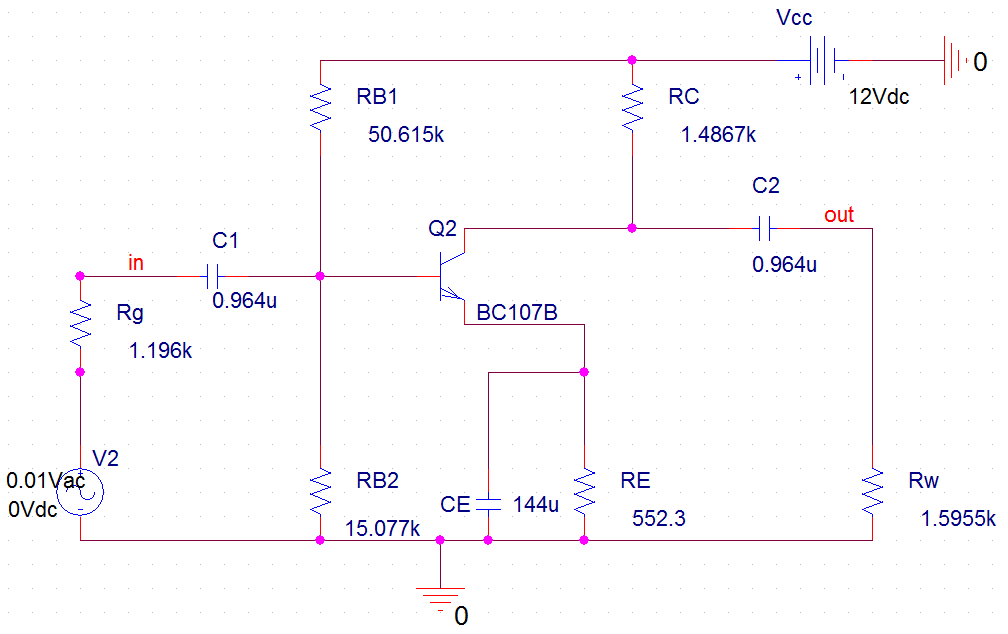
\includegraphics[width=0.8\textwidth]{schemat.png}
  \caption{Schemat do symulacji projektowanego układu}
\end{figure}

\newpage
\section{Wyniki symulacji}

\begin{figure}[h]
  \center
  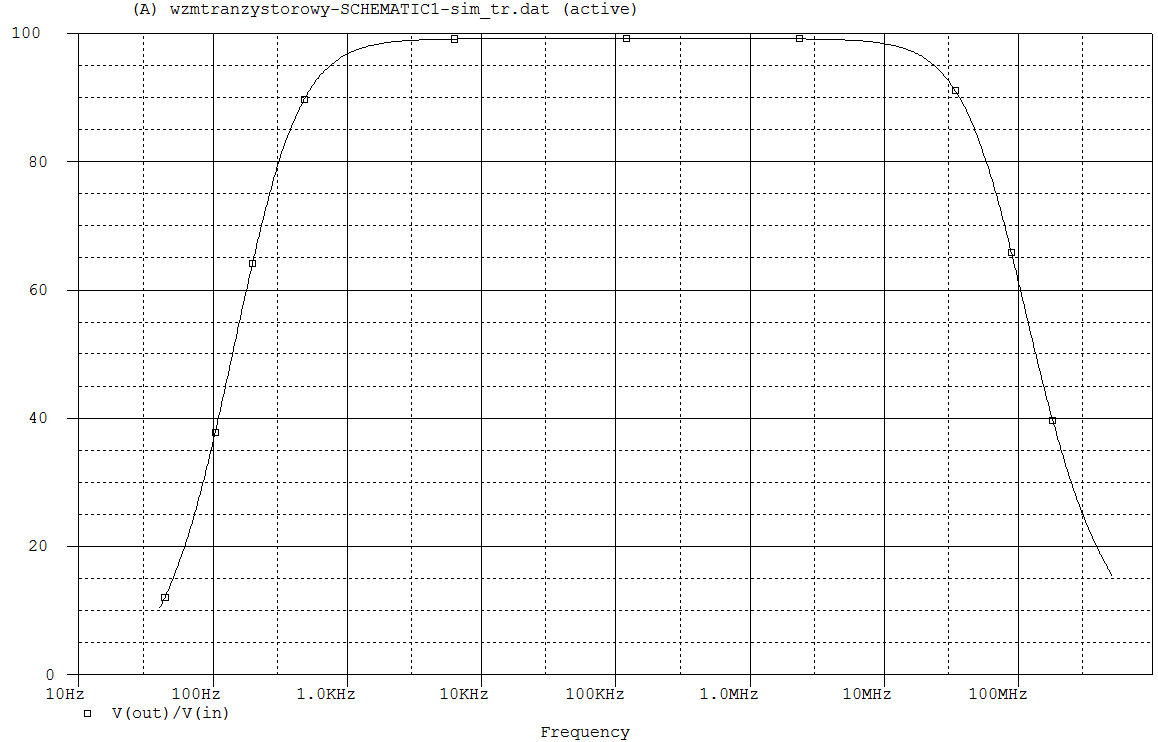
\includegraphics[width=0.81\textwidth]{sim1.png}
  \caption{Charakterystyka częstotliowściowa wzmacniacza, $C_E = 144uF$}
  
    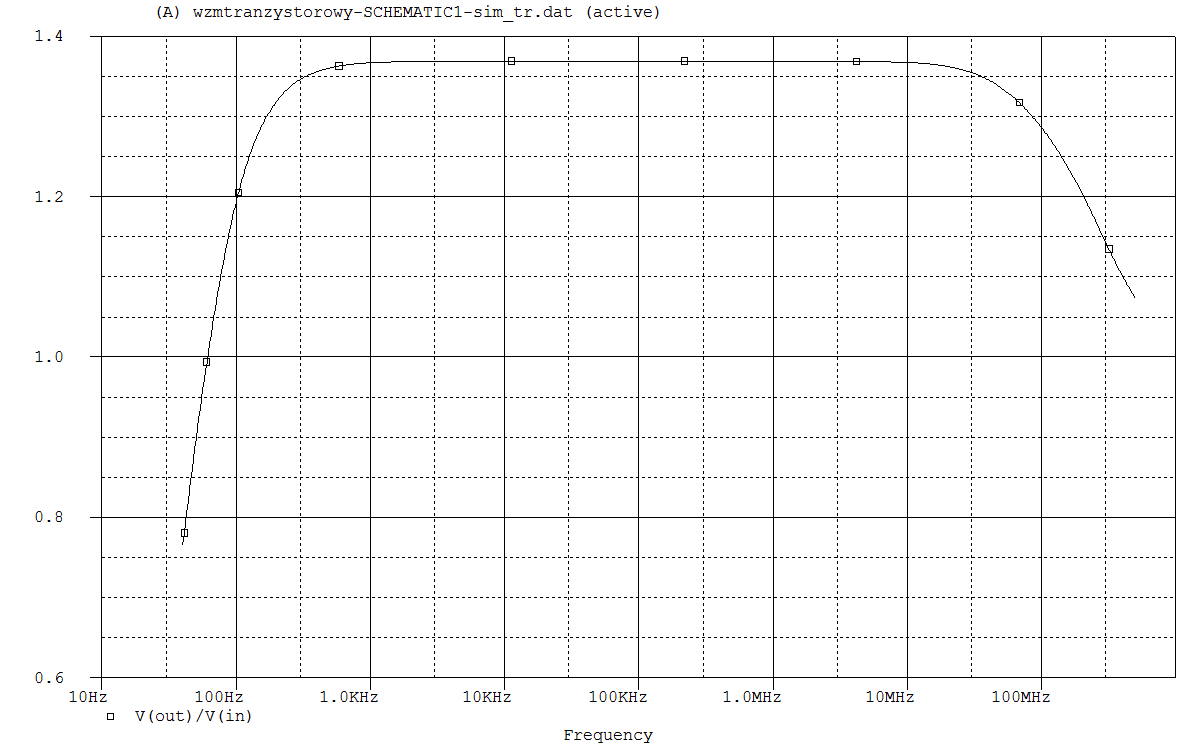
\includegraphics[width=0.81\textwidth]{sim2.png}
  \caption{Charakterystyka częstotliowściowa wzmacniacza, $C_E = 0$}
\end{figure}


\pagebreak
%%%%%%%%%%%%%%%%%%%%%%%%%%%%%%%%%%%%%%%%%%%%%%%%%%%%%%%%%%%%%%%%%%%%%%%%%%%%%%%%%%%%%%%%%%%%%%%%%%%%%%%%%%%%%%%%%%%%%%%%%%%%%%%%%%%%%%%%%%%%%%%%%%%%
%%%%%%%%%%%%%%%%%%%%%%%%%%%%%%%%%%%%%%%%%%%%%%%%%%%%%%%%%%%%%%%%%%%CZĘŚĆ LABORATORYJNA%%%%%%%%%%%%%%%%%%%%%%%%%%%%%%%%%%%%%%%%%%%%%%%%%%%%%%%%%%%%%%
%%%%%%%%%%%%%%%%%%%%%%%%%%%%%%%%%%%%%%%%%%%%%%%%%%%%%%%%%%%%%%%%%%%%%%%%%%%%%%%%%%%%%%%%%%%%%%%%%%%%%%%%%%%%%%%%%%%%%%%%%%%%%%%%%%%%%%%%%%%%%%%%%%%%
\section{Część laboratoryjna}
\subsection{Charakterystyka częstotliwościowa wzmacniacza}

\begin{table}[ht]
  \begin{center}
  \begin{tabular}{|r|r|r|r|r|r|r|r|r|}
    \hline
    \multicolumn{9}{|c|}{\textbf{$\mathbf{C_E = 144uF}, \quad \mathbf{R_w=1.596[k\Omega]}$}} \\ \hline
    \multicolumn{4}{|c|}{$\mathbf{R_g = 1.196[k\Omega]}$} & & \multicolumn{4}{c|}{$\mathbf{R_g = 0}$} \\ \cline{1-4} \cline{6-9}
    $\mathbf{f[kHz]}$ & $\mathbf{U_{we}[mV]}$ & $\mathbf{U_{wy}[V]}$ & $\mathbf{K_{U12}[\frac{V}{V}]}$ & & $\mathbf{f[kHz]}$ & $\mathbf{U_{we}[mV]}$ & $\mathbf{U_{wy}[V]}$ & $\mathbf{K_{USK}[\frac{V}{V}]}$ \\ \cline{1-4} \cline{6-9}
    0,25 & 74,0 & 0,398 & 53,73 & & 0,15 & 72,8 & 0,210 & 28,85 \\ \cline{1-4} \cline{6-9}
    0,35 & 73,6 & 0,448 & 60,87 & & 0,35 & 74,0 & 0,272 & 36,76 \\ \cline{1-4} \cline{6-9}
    0,48 & 73,6 & 0,500 & 67,93 & & 0,55 & 73,0 & 0,288 & 39,45 \\ \cline{1-4} \cline{6-9}
    0,60 & 73,0 & 0,545 & 74,66 & & 5,00 & 74,4 & 0,300 & 40,32 \\ \cline{1-4} \cline{6-9}
    30,00 & 72,5 & 0,569 & 78,48 & & 70,00 & 73,6 & 0,300 & 40,76 \\ \cline{1-4} \cline{6-9}
    150,00 & 72,4 & 0,568 & 78,48 & & 85,00 & 73,6 & 0,300 & 40,76 \\ \cline{1-4} \cline{6-9}
    330,00 & 74,0 & 0,550 & 74,32 & & 220,00 & 74,0 & 0,272 & 36,76 \\ \cline{1-4} \cline{6-9}
    525,00 & 72,4 & 0,506 & 69,89 & & 440,00 & 73,0 & 0,212 & 29,04 \\ \cline{1-4} \cline{6-9}
    840,00 & 73,6 & 0,442 & 60,05 & & \multicolumn{4}{c|}{-} \\ \cline{1-4} \cline{6-9}
    1000,00 & 72,0 & 0,392 & 54,44 & & \multicolumn{4}{c|}{-} \\ \hline
    \multicolumn{9}{|c|}{$\mathbf{R_w = \infty}$} \\ \hline
    150,00 & 72,2 & 1,050 & - & & 85,00 & 73,0 & 0,544 & - \\ \hline
    \multicolumn{9}{|c|}{\textbf{$\mathbf{C_E = 0}, \quad \mathbf{R_w=1.596[k\Omega]}$}} \\ \hline
    0,06 & 1,44 & 0,138 & 0,96 & & 0,06 & 1,44 & 0,122 & 0,85 \\ \cline{1-4} \cline{6-9}
    0,22 & 1,44 & 0,180 & 1,25 & & 0,09 & 1,44 & 0,144 & 1,00 \\ \cline{1-4} \cline{6-9}
    50,00 & 1,44 & 0,200 & 1,39 & & 0,15 & 1,44 & 0,160 & 1,11 \\ \cline{1-4} \cline{6-9}
    130,00 & 1,44 & 0,200 & 1,39 & & 10,00 & 1,44 & 0,172 & 1,19 \\ \cline{1-4} \cline{6-9}
    460,00 & 1,44 & 0,180 & 1,25 & & 30,00 & 1,44 & 0,172 & 1,19 \\ \cline{1-4} \cline{6-9}
    1000,00 & 1,44 & 0,142 & 0,99 & & 515,00 & 1,44 & 0,158 & 1,10 \\ \cline{1-4} \cline{6-9}
    \multicolumn{4}{|c|}{-} & & 785,00 & 1,44 & 0,140 & 0,97 \\ \cline{1-4} \cline{6-9}
    \multicolumn{4}{|c|}{-} & & 1150,00 & 1,44 & 0,120 & 0,83 \\ \hline
    \multicolumn{9}{|c|}{$\mathbf{R_w = \infty}$} \\ \hline
    130,00 & 1,46 & 0,60 & - & & 30 & 1,44 & 0,330 & - \\ \hline

  \end{tabular}
  \end{center}
  
\end{table}


%\pagebreak
%%%%%%%%%%%%%%%%%%%%%%%%%%%%%%%%%%%%%%%%%%%%%%%%%%%%%%%%%%%%%%%%%%%%%%%%%%%%%%%%%%%%%%%%%%%%%%%%%%%%%%%%%%%%%%%%%%%%%%%%%%%%%%%%%%%%%%%%%%%%%%%%%%%%

\begin{figure}[h!]
  \begin{center}
  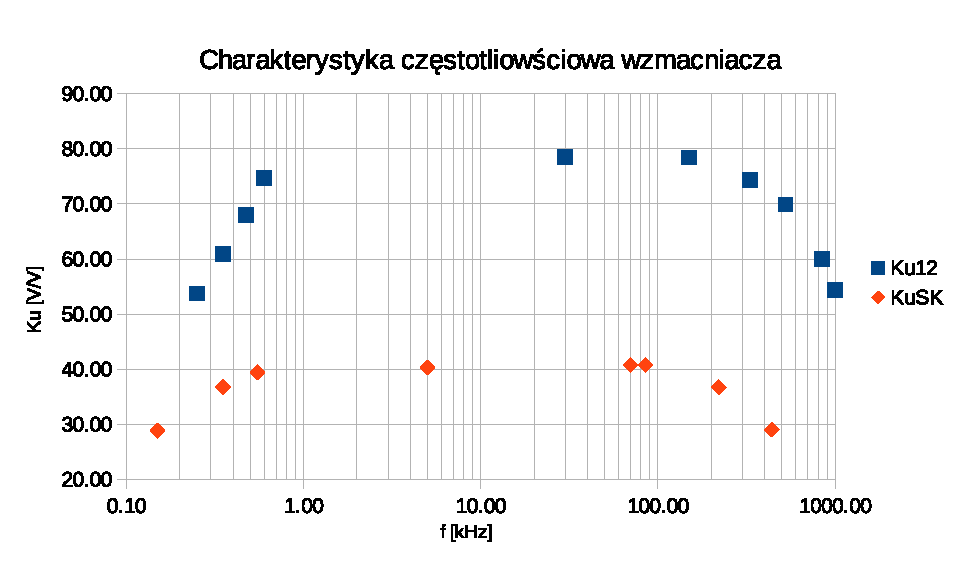
\includegraphics[width=0.85\textwidth]{g1.eps}
  \caption{Charakterystyka częstotliowśiowa wzmacniacza przy $C_E = 144uF$}
  \end{center}

  Z danych pomiarowych zamieszczonych w tabeli oraz powyższego wykresu możemy odczytać:
  \begin{itemize}
  \item $K_{U12} = 78.48 \frac{V}{V}$
  \item $K_{USK} = 40.76 \frac{V}{V}$
  \item Otrzymane na podstawie symulacji $K_{U12}=K_{USK}\approx 100\frac{V}{V}$
  \item $fd_{12} \approx 0.25[kHZ]$
  \item $fd_{SK} \approx 0.15[kHz]$
  \item $fd_{sim} \approx 0.2[kHz]$
  \item $fg_{12} \approx 1000[kHZ]$
  \item $fg_{SK} \approx 440[kHz]$
  \item $fg_{sim} \approx 80000[kHz]$


  \end{itemize}
    $ $ \newline
$ $ \newline
$ $ \newline
\end{figure}


\begin{figure}[h!]
  \begin{center}
  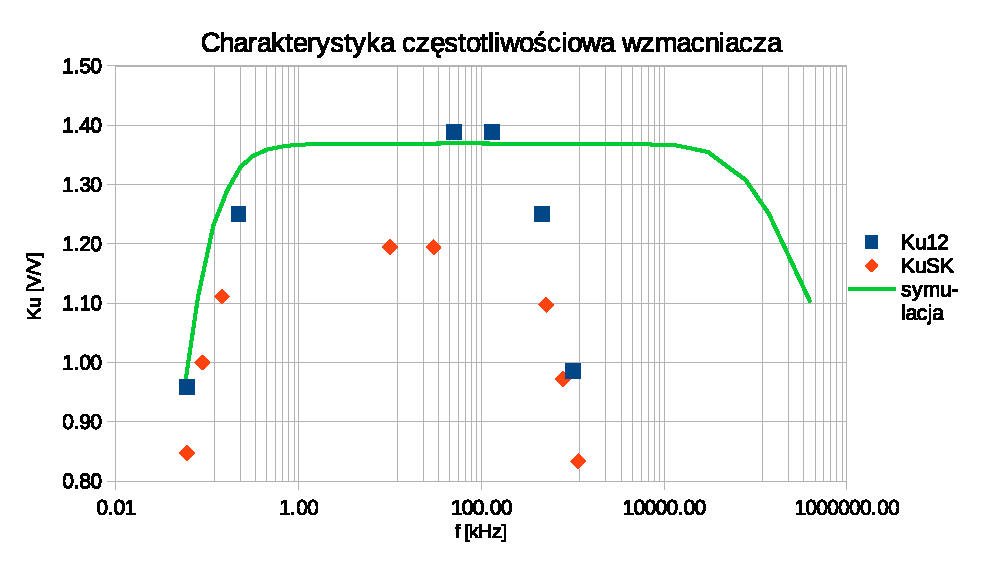
\includegraphics[width=0.85\textwidth]{g2.eps}
  \caption{Charakterystyka częstotliowśiowa wzmacniacza przy $C_E = 0$}
  \end{center}
  
    Z danych pomiarowych zamieszczonych w tabeli oraz powyższego wykresu możemy odczytać:
  \begin{itemize}
  \item $K_{U12} = 1.39 \frac{V}{V}$
  \item $K_{USK} = 1.19 \frac{V}{V}$
  \item Otrzymane na podstawie symulacji $K_{U12}=K_{USK}\approx 1.37\frac{V}{V}$
  \item $fd_{12} \approx 0.06[kHZ]$
  \item $fd_{SK} \approx 0.06[kHz]$
  \item $fd_{sim} \approx 0.06[kHz]$
  \item $fg_{12} \approx 1000[kHZ]$
  \item $fg_{SK} \approx 1150[kHz]$
  \item $fg_{sim} > 40000[kHz]$
  
  \end{itemize}
      $ $ \newline
$ $ \newline
$ $ \newline
$ $ \newline
$ $ \newline
\end{figure}




%%%%%%%%%%%%%%%%%%%%%%%%%%%%%%%%%%%%%%%%%%%%%%%%%%%%%%%%%%%%%%%%%%%%%%%%%%%%%%%%%%%%%%%%%%%%%%%%%%%%%%%%%%%%%%%%%%%%%%%%%%%%%%%%%%%%%%%%%%%%%%%%%%%%

%%%%%%%%%%%%%%%%%%%%%%%%%%%%%%%%%%%%%%%%%%%%%%%%%%%%%%%%%%%%%%%%%%%%%%%%%%%%%%%%%%%%%%%%%%%%%%%%%%%%%%%%%%%%%%%%%%%%%%%%%%%%%%%%%%%%%%%%%%%%%%%%%%%%

\newpage
\section {Wnioski}

\begin{itemize}
  \item Na podstawie Rysunku nr 4 widzimy, iż zasilacz pracuje zgodnie z oczekiwaniami teoretycznymi, ponieważ dla 
	napięcia nominalnego $U_{we} = 9V$ na wyjściu otrzymujemy zadane napięcie ok. 6V.
  \item Wykres z rysunku nr 5 wskazuje na to, że układ został zaprojektowany i wykonany zgodnie z założeniami
	projektowymi, gdyż dla wartości od kilkudziesięciu mA do ok. 225mA natężenia prądu wyjściowego 
	układ utrzymuje zadane napięcie wyjściowe na poziomie ok. 6V. Zakres ten jest o ok. 25mA mniejszy
	od założonego $I_{max} = 250mA$. Wynika to najprawdopodobniej z użycia nieco innych wartości
	elementów niż zakłdają obliczenia projektowe.
  \item Sprawność wyrysowana w zależności od natężenia prądu wyjściowego na rystunku nr 6 przyjmuje 
	wartości na poziomie 0.7 - 0.8 co możemy uznać za wartości mieszczące się w normach tego typu układów.
\end{itemize}

\end{document}
